\chapter{Basic Datastructures}

% the problem of working with individual values

\section{Types}

\subsection{Complex Types}

\subsection{Reference Types}

\section{Structured Data}

\subsection{Colors}

% light as a spectrum
\defix{Light} is made up of photons, and each \idx{photon}{Photon} has a wavelength. The \defi{wavelength}{Wavelength} of the photons determines which color our eyes will observe. A wavelength of 380nm is \idx{violet}{Violet} and one of 740nm is \idx{red}{Red}. In between these you have all the colors of the \idx{rainbow}{Rainbow}, in the order of the rainbow. Coincidence? Just outside of the \idx{visible spectrum}{Spectrum!Visible}, you will find \idx{infra-red}{Infra-red} and \idx{ultra-violet}{Untra-violet}. Our eyes are, however, constantly bombarded by photons, so in reality we always observe a distribution across this spectrum. Our \idx{eyes}{Eye}, though only has three (or four) tunings of receptors. These, roughly corresponds to red, green and blue. So, your eyes (and \idx{brains}{Brain}) need to do a lot of interpretation.

% computer representation
In a computer, colors are typically \idx{represented}{Representation!Color} using three values; one for red intensity, one for green intensity, and one for blue intensity. That somehow matches the model of our eyes \ldots We say that these are the \textsl{components} of the color. There is a number of ways to express such an \idx{intensity}{Intensity}. It seem natural to use a number between 0 and 100, or perhaps a number between 0.0 and 1.0. However, due to the way processors work on integers, these boundaries are not particularly special. Typically, a byte is use to represent each component of the color. That means that we have the ability to express $2^8=256$ different intensities of each component, or a total of $256^3=16777216$ different colors. The value zero is used to represent complete \idx{darkness}{Darkness}. Full intensity is then the value 255.

% figure: color cube
\begin{figure}[tbp]
  \begin{center}
  \scalebox{1.0}{
    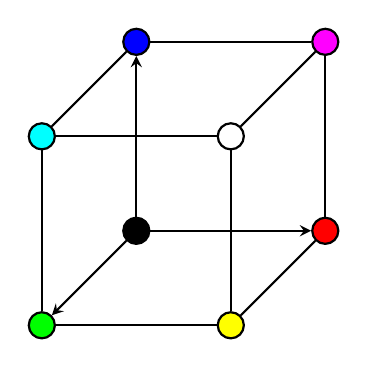
\begin{tikzpicture}
      \newcommand{\dist}[0]{24mm}
      \newcommand{\zdist}[0]{12mm}
      
      \tikzstyle{node}=[
        draw,
        circle,
        minimum height=0.2cm,
        minimum width=0.2cm,
        anchor=center,
        thick
      ]
      \tikzstyle{arrow} = [thick,->,>=stealth, draw=black]
      \tikzstyle{line} = [thick, draw=black]
      
      \definecolor{mycyan}{rgb}{0.0,1.0,1.0}
      \definecolor{mymagenta}{rgb}{1.0,0.0,1.0}
      \definecolor{myyellow}{rgb}{1.0,1.0,0.0}
      
      \node[node, fill=blue]      (blue)    at (0    , 0) {};
      \node[node, fill=mymagenta] (magenta) at (\dist, 0) {};
      \node[node, fill=black]     (black)   at (0    , -\dist) {};
      \node[node, fill=red]       (red)     at (\dist, -\dist) {};
      \node[node, fill=mycyan]   (cyan)   at (0-\zdist    , 0-\zdist) {};
      \node[node, fill=white]    (white)  at (\dist-\zdist, 0-\zdist) {};
      \node[node, fill=green]    (green)  at (0-\zdist    , -\dist-\zdist) {};
      \node[node, fill=myyellow] (yellow) at (\dist-\zdist, -\dist-\zdist) {};
      
      \draw[arrow] (black) -- (red);
      \draw[arrow] (black) -- (green);
      \draw[arrow] (black) -- (blue);
      \draw[line] (blue) -- (magenta);
      \draw[line] (blue) -- (cyan);
      \draw[line] (red) -- (magenta);
      \draw[line] (red) -- (yellow);
      \draw[line] (green) -- (yellow);
      \draw[line] (green) -- (cyan);
      \draw[line] (white) -- (cyan);
      \draw[line] (white) -- (magenta);
      \draw[line] (white) -- (yellow);
    \end{tikzpicture}
  }
\end{center}

  \caption{RGB color cube.}
  \label{fig:primdata:struct:color}
\end{figure}

% color spaces
This constitutes a \defi{color space}{Color!Space} whereby all colors fit within a \idx{color cube}{Color!Cube} spanned by the red, green and blue color vectors. Hence, it is named the \idxx{RGB} color space. Figure \ref{fig:primdata:struct:color} depicts this space. It is a direct fit for how \idx{GPUs}{GPU} represent \idx{images}{Image}. Other color spaces exist though, and there are good reasons for their existence. Other popular color spaces include \idxx{HSV} (which is shaped like a cylinder) and \idxx{XYZ} (which is shaped like an tongue). Formulas exists for \idx{converting}{Color!Space!Converting} between these. Each of these color spaces represents practical simplifications of what light really is.

\csharpsubsection{\csharp}

% value type through struct, reference type through class

\begin{syntaxfloat}
  \begin{syntax}[[xshift=22mm]concept.west]{vismod}
  \SyntaxWestSplit{MainWest}
  \SyntaxEastSplit{MainEast}
  
  \node[terminal] (ruleIa) at ($(begin)!0.5!(end)$) {public};
  
  \draw[path] (begin)--(ruleIa)--(end);
\end{syntax}

\begin{syntax}[[xshift=22mm]concept.west]{global-var}
  \SyntaxWestSplit{MainWest}
  \SyntaxEastSplit{MainEast}
  
  \node[sequence,anchor=north] () at ([yshift=\syntaxrulenodeheight-0.8pt*3]$(begin.east)!0.5!(end.west)$) {
    \node[nonterminal] (ruleIa) {vismod};
    &
    \node[nonterminal] (ruleIb) {type};
    &
    \node[terminal]    (ruleIc) {name};
    &
    \node[terminal]    (ruleId) {=};
    &
    \node[nonterminal] (ruleIe) {expr};
    &
    \node[terminal]    (ruleIf) {;};
    \\
    \node[nonterminal] (ruleIIa) {vismod};
    &
    \node[nonterminal] (ruleIIb) {type};
    &
    \node[terminal]    (ruleIIc) {name};
    &
    &
    &
    \node[terminal]    (ruleIId) {;};
    \\
  };
  
  \draw[path] (begin)--(ruleIa)--(ruleIb)--(ruleIc)--(ruleId)--(ruleIe)--(ruleIf)--(end);
  \draw[path] (begin) to[-|-] ([xshift=1cm,yshift=-1*(\syntaxruledist+0.8pt*3)]begin.east)--(ruleIIa)--(ruleIIb)--(ruleIIc)--(ruleIId)--([xshift=-1cm,yshift=-1*(\syntaxruledist+0.8pt*3)]end.west) to[-|-] (end);
\end{syntax}

\begin{syntax}[[xshift=24mm]concept.west]{global-vars}
  \SyntaxWestSplit{MainWest}
  \SyntaxEastSplit{MainEast}
  
  \node[sequence] () at ([yshift=\syntaxruledist-0.8pt*3]$(begin)!0.5!(end)$) {
    \\
    \node[nonterminal]    (ruleIa) {global-var};
    \\
  };
  
  \draw[path] (begin)--(end);
  \draw[path] (begin) to[-|-] (ruleIa) to[-|-] (end);
  \draw[path] (ruleIa)
            -|([xshift= 0.5*\syntaxruledist,yshift=0.4*\syntaxruledist]ruleIa.east)
            |-(                            [yshift=0.8*\syntaxruledist]ruleIa.center)
            -|([xshift=-0.5*\syntaxruledist,yshift=0.4*\syntaxruledist]ruleIa.west)
            |-(ruleIa);
\end{syntax}

\begin{syntax}[[xshift=22mm]concept.west]{class}
  \SyntaxWestSplit{MainWest}
  \SyntaxEastSplit{MainEast}
  
  \node[sequence,anchor=north] () at ([yshift=\syntaxrulenodeheight-0.8pt*3]$(begin.east)!0.5!(end.west)$) {
    \node[terminal]    (ruleIa) {class};
    &
    \node[terminal]    (ruleIb) {name};
    &
    \node[terminal]    (ruleIc) {\{};
    &
    \node[nonterminal] (ruleId) {global-vars};
    &
    \node[terminal]    (ruleIe) {\}};
    \\
  };
  
  \draw[path] (begin)--(ruleIa)--(ruleIb)--(ruleIc)--(ruleId)--(ruleIe)--(end);
\end{syntax}

  \caption{Structured data}
  \label{syntax:data:struct}
\end{syntaxfloat}

\section{Sequences in Data}

\subsection{Arrays}

\subsubsection{Indexing}

% calculation, this is why most languages agree that arrays start at zero

\subsubsection{Multidimensional Arrays}

\subsection{Linked Lists}

% head and tail

\subsection{Doubly Linked Lists}

\subsection{Looping Sequences}

\subsection{Nesting}

\subsection{Points}

\section{Enumerations}

\subsection{State Machines}

\subsection{String Parsing Example}

\section{Case: Dynamic Arrays} % TODO: should this go into the function chapter?

% problem: arrays have a static size

% observation: a variable only references an array

% solution: Wrap the array in a struct

\csharpsubsection{\csharp}

\begin{syntaxfloat}
  \begin{syntax}[[xshift=24mm]concept.west]{names}
  \SyntaxWestSplit{MainWest}
  \SyntaxEastSplit{MainEast}
  
  \node[sequence] () at ([yshift=-0*\syntaxruledist]$(begin)!0.5!(end)$) {
    \node[nonterminal]    (ruleIa) {name};
    \\
  };
  
  \node[sequence] () at ([yshift=1*\syntaxruledist]$(begin)!0.5!(end)$) {
    \node[terminal]    (ruleIIa) {,};
    \\
  };
  
  \draw[path] (begin)--(ruleIa)--(end);
  \draw[path] (ruleIa)
            -|([xshift= 0.5*\syntaxruledist,yshift=0.4*\syntaxruledist]ruleIa.east)
            |-(                            [yshift=0.0*\syntaxruledist]ruleIIa)
            -|([xshift=-0.5*\syntaxruledist,yshift=0.4*\syntaxruledist]ruleIa.west)
            |-(ruleIa);
\end{syntax}

\begin{syntax}[[xshift=22mm]concept.west]{enum}
  \SyntaxWestSplit{MainWest}
  \SyntaxEastSplit{MainEast}
  
  \node[sequence,anchor=north] () at ([yshift=\syntaxrulenodeheight-0.8pt*3]$(begin.east)!0.5!(end.west)$) {
    \node[terminal]    (ruleIa) {enum};
    &
    \node[terminal]    (ruleIb) {name};
    &
    \node[terminal]    (ruleIc) {\{};
    &
    \node[nonterminal] (ruleId) {names};
    &
    \node[terminal]    (ruleIe) {\}};
    \\
  };
  
  \draw[path] (begin)--(ruleIa)--(ruleIb)--(ruleIc)--(ruleId)--(ruleIe)--(end);
\end{syntax}

  \caption{Enums}
  \label{syntax:data:enum}
\end{syntaxfloat}

